% --------------------- VARIABLEN -------------------------

\newcommand{\COURSE}{Physik und Materialwissenschaften\\ Praktikum Physik \\}
\newcommand{\SEMESTER}{Elektro- und Informationstechnik II}
\newcommand{\STUDENT}{Maximilian Spahn\\ und\\Benjamin Langer}

\newcommand{\HEADDING}{Praktikum Physik}
\newcommand{\SUBHEADDING}{Versuch 4.1: Wärmeausdehnung und Mischtemperatur}

% ------------------- DEFINITIONEN -----------------------

\documentclass[a4paper]{scrartcl}

\usepackage[utf8]{inputenc}
\usepackage[ngerman]{babel}
\usepackage{amsmath}
\usepackage{amssymb}
\usepackage{color}
\usepackage{tikz}
\usepackage{float}
\usetikzlibrary{arrows,decorations.markings}
\usepackage{tabularx}
\usepackage{fancybox}
\usepackage{pgfplots}
\usepackage[colorlinks=false,linkcolor=black,urlcolor=blue,bookmarks,bookmarksopen=true]{hyperref}
\usepackage{geometry}
\usepackage{fancyhdr}

\usepackage[page]{totalcount}

%Größe der Ränder setzen
\geometry{a4paper,left=2cm, right=2cm, top=3cm, bottom=2cm, headheight=8cm}

%Kopf- und Fußzeile
\pagestyle {fancy}
\fancyhf{}
\fancyhead[L]{\STUDENT}
\fancyhead[C]{\COURSE}
\fancyhead[R]{\today}

\fancyfoot[L]{\SEMESTER}
\fancyfoot[C]{}
\fancyfoot[R]{Seite \thepage /\pageref{LastPage}}

%Formatierung der Überschrift, hier nichts ändern
\def\header#1#2{
  \begin{center}
    {\Large #1}\\
    {#2}
  \end{center}
}

\numberwithin{equation}{subsection}

\nocite{*}
\bibliographystyle{plainurl}

\setlength\parindent{0pt}

% ----------------------- DOCUMENT ---------------------------

\begin{document}

\vspace{10pt}
\header{\HEADDING}{\SUBHEADDING}

\tableofcontents

\newpage

\section{Einleitung}
Die beiden Versuche, welche in dieser Ausarbeitung behandelt werden, beschäftigen sich mit einigen Grundsätzen der Thermodynamik. Dabei geht der erste Versuch besonders auf die Wärmeausdehnung, in Abhängigkeit der Temperatur bei verschieden Materialien ein. In der Theorie wird herbei der chemische Zusammenhang für dieses Verhalten erläutert.
Der Zweite Versuch verdeutlicht die Wärmekapazität von Stoffen. Dies wird durch das Ermitteln der Mischtemperatur von Eis und Wasser und den entsprechenden theoretischen Zusammenhängen gezeigt. 

\newpage
\section{Theorie}
\subsection{Wärmeausdehnung}

Wenn man ein Stück eines Materials mit bestimmten geometrischen Abmessungen erhitzt oder abkühlt, dehnt sich dieses aus oder zieht sich entsprechend zusammen. Dies wird als Wärmeausdehnung bezeichnet. 
Dieser Effekt tritt sowohl bei festen, flüssigen, aber auch gasförmigen Stoffen auf. Im folgenden wird aber verstärkt die lineare Ausdehnung von Feststoffen betrachtet. \cite{hering} \\

Zwar dehnt sich ein Körper beim Erwärmen in alle drei Dimensionen gleichzeitig aus, dennoch wird hier nur die Ausdehnung in eine Richtung betrachtet, da die Ausdehnung in allen Richtungen gleich ist und sich die Längenänderung eines langen Stabes einfacher betrachten lässt. Da die Längenänderung proportional zur Anfangslänge ist, lässt sich bei einer größeren Anfangslänge auch eine größere Längenänderung erwarten (und einfacher genau messen). \cite{werk}

\begin{figure}[H]
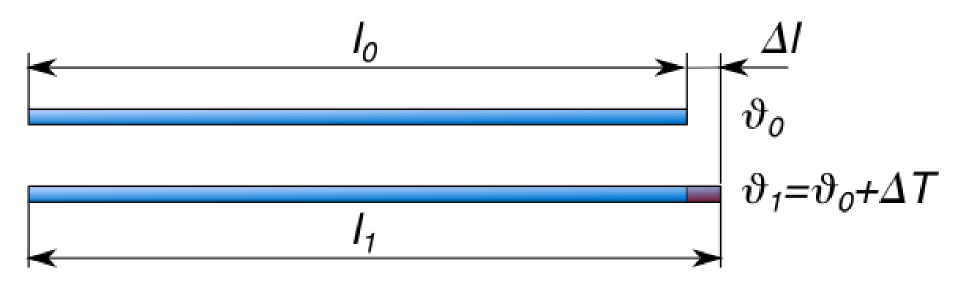
\includegraphics[width=12cm]{Abbildungen/lineare_ausdehnung}
\centering
\caption{Lineare Längenänderung eines langen Stabes \protect\footnotemark}
\centering
\label{fig:lineare-ausdehnung}
\end{figure}

\footnotetext{\url{https://de.wikipedia.org/wiki/W\%C3\%A4rmeausdehnung\#/media/Datei:Linia_dilato.png}}

Die Längenänderung ergibt sich aus den interatomaren Abständen der Atome. Diese entstehen aus der Überlappung der Atomorbitale. Atomorbitale bescheiben Bereiche um Atome in welchen sich Elentronen aufhalten können. Diese Elektronen sind als Bindungselektronen interesant. So ermöglichen die negativ geladenen Elektronen zwischen den postiven Kernen, welche sich eigentlich abstoßen müssten, dass eine Bindung erstehen kann.
Bei der Bindung haben die Atome dadurch einen bestimmten Abstand. Dieser Abstand ist erreicht, wenn die Kraft der Abstoßung der Atomkerne mit der Anziehungskraft beider Kerne zu den Elektronen in der Mitte im Gleichgewicht ist. Wenn die Kräfte im Gleichgewicht sind, haben die Elektronen einen stabilen Zustand im Energieminimum.
Durch die hinzugefügte Wärmeenergie, wird dieses Gleichgewicht verschoben und der ideale Abstand, in welchem das Gleichgewicht erreicht ist, wird größer. \cite{werk}

\begin{figure}[H]
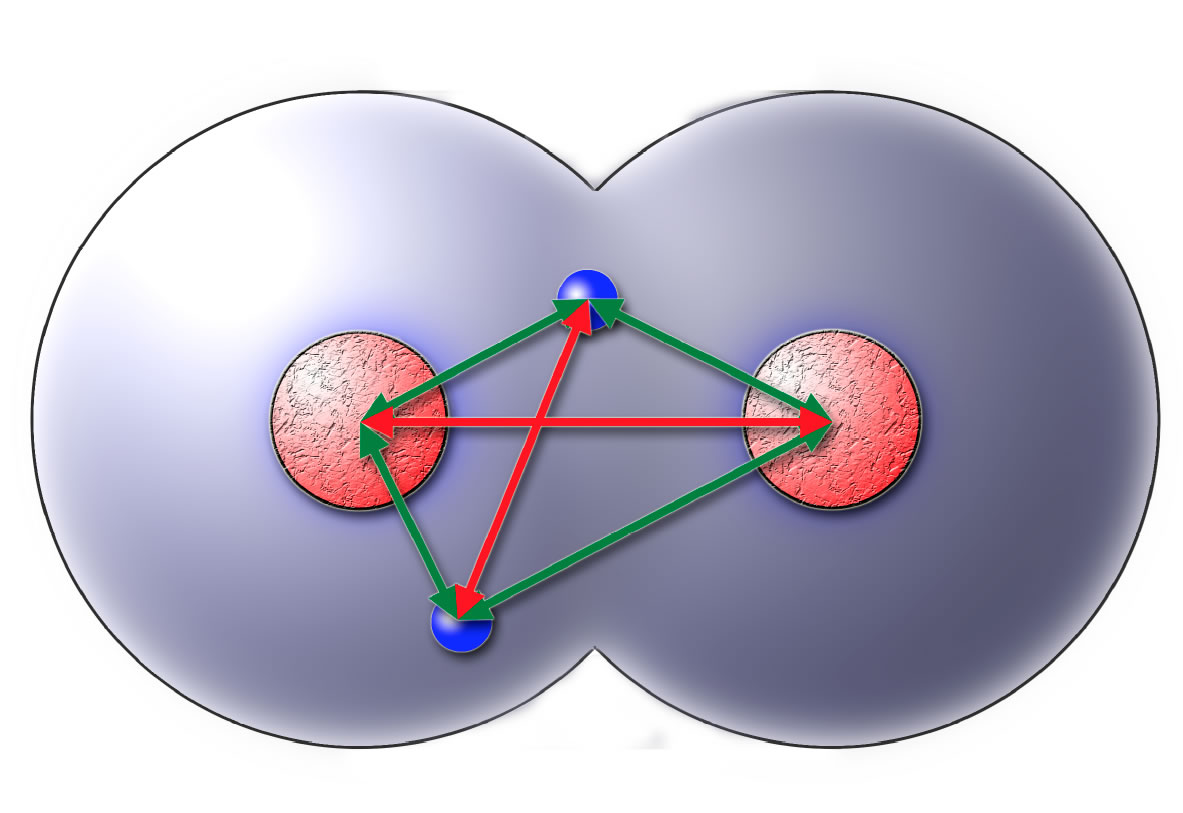
\includegraphics[width=12cm]{Abbildungen/bindungselektronen}
\centering
\caption{Bindungselektronen zwischen zwei Atomkernen \protect\footnotemark}
\centering
\label{fig:bindungselektronen}
\end{figure}

\footnotetext{\url{http://www.u-helmich.de/che/0809/05-molek/mol02.html}}

\begin{figure}[H]
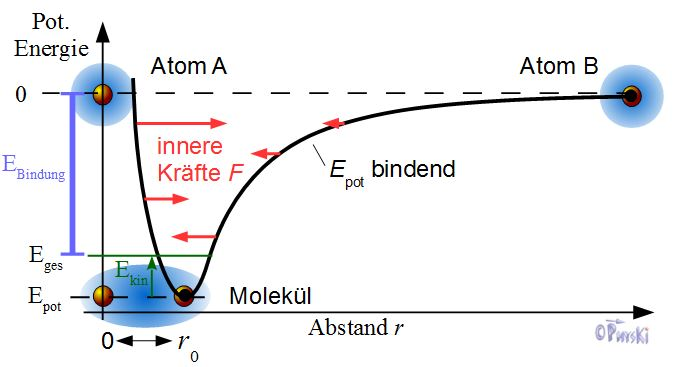
\includegraphics[width=12cm]{Abbildungen/bindungsenergie}
\centering
\caption{interatomares Potential \protect\footnotemark}
\centering
\label{fig:bindungsenergie}
\end{figure}

\footnotetext{\url{https://www2.physki.de/PhysKi/index.php/Datei:Bindungsenergie.jpg}}
\newpage

Der Zusammenhang zwischen Temperaturänderung und Längenänderung ist linear und kann durch folgende Gleichung beschrieben werden. \cite{anl}

\begin{align}
\Delta L = \alpha \cdot L_0 \cdot \Delta T
\end{align}

mit 

\begin{align*}
\Delta L	 \qquad 	& \text{Längenänderung} \\
\alpha	 \qquad 	& \text{linearer Ausdehnungskoeffizient in $\frac{1}{K}$} \\
L_0 		 \qquad 	& \text{Anfangslänge} \\
\Delta T	 \qquad 	& \text{Temperaturdifferenz in $K$}
\end{align*}

\subsection{Mischtemperatur}

Werden 2 Stoffe, unterschiedlicher Temperatur gemischt oder kommen in Kontakt, so gibt der Körper mit höherer Temperatur, Wärme an den Körper mit niedriger Temperatur ab. Dabei gilt der Energie Erhaltungssatz. \\

Die Wärmeenergie eines Körpers bzw. deren Änderung $\Delta Q$ hängt ab von der Temperaturänderung $\Delta T$, seiner Masse $m$ und seiner Wärmekapazität $c$. \cite{anl}

\begin{align}
\Delta Q = m \cdot c \cdot \Delta T
\end{align}

Die Wärmekapazität ist von Material zu Material unterschiedlich und hängt von der Anzahl der Bindungen und deren Freiheitsgraden ab.\\

Wird einem Material Energie hinzugefügt, erhöht sich also dessen Temperatur. Nur bei den Übergängen der Aggregatzustände muss zuerst eine Übergangsenergie aufgewendet werden, bei welcher sich die Atome neu anordnen und sich die Temperatur nicht verändert. 
Diese Zusammenhänge sind in den folgenden Gleichungen dargestellt: \cite{anl}

\begin{align}
\Delta Q_S &= m \cdot q_S \\
\Delta Q_V &= m \cdot q_V
\end{align}

mit 

\begin{align*}
q_S \qquad 	& \text{spezifische Schmelzwärme} \\
q_V	\qquad 	& \text{spezifische Verdampfungswärme}
\end{align*}

Werden zwei unterschiedliche Stoffe/Flüssigkeiten mit den Massen: $m_1$ bzw. $m_2$
und den Anfangstemperaturen $T_1$ und $T_2$ zusammengemischt, ermittelt man die Mischtemperatur
$T_M$ anhand der jeweiligen spezifischen Wärmekapazitäten $c_1$ bzw. $c_2$ wie folgt. \cite{anl}

\begin{align}
T_M = \frac{c_1 \cdot m_1 \cdot T_1 + c_2 \cdot m_2 \cdot T_2}{c_1 \cdot m_1 + c_2 \cdot m_2}
\end{align}

(Die Herleitung aufgrund des Energieerhaltungssatzes wird in der häuslichen Vorarbeit behandelt)

\newpage
\section{Häusliche Vorarbeit}
\subsection{Teil A: Wärmeausdehnung}
\subsubsection{3.2.2: Wärmeausdehnung auf atomarer Ebene}
Wie bereits in dem Theorie Teil beschrieben, hängt die Längenänderung von Feststoffen bei Temperaturänderung von der Änderung der Bindungsenergie der Atome ab. Durch die zusätzliche Energie haben die Atome innerhalb ihrer regelmäßigen Anordnung mehr Platz zu schwingen. Bei 0 K sind die Atome fest in einem Abstand, bei welchem die Bindungsenergie am geringsten ist. Durch die zusätzliche Wärmeenergie können die Atome um diesen Abstand schwingen und nehmen so mehr Platz ein.

\subsubsection{3.2.3: 3-dimensionale Objekte}
Materialien dehnen sich in alle drei Dimensionen gleichmäßig aus. Die Formel für die Längenänderung gilt unabhängig für alle drei Dimensionen. Da die alle drei Richtungen von der Temperaturänderung betroffen sind und den selben Ausdehnungskoeffizient haben ist die Längenänderung in allen Richtungen gleichmäßig vorhanden. Da sich die Längenänderung proportional zur Anfangslänge des Körpers verhält, kann es einem, bei sehr langen Objekten vorkommen, als würde sich nur eine Richtung ausdehnen.

\subsection{Teil B: Mischtemperatur}
\subsubsection{4.2.2: Herleitung Mischtemperatur}

Die Mischtemperatur $T_M$ lässt sich über den Energieerhaltungssatz herleiten. So ist die Energie des Gemischs die Summe der Energien der beiden Flüssigkeiten.

\begin{align*}
Q_{\textit{ges}} = Q_1 + Q_2
\end{align*}

Nun wird die Formel für die gespeicherte Wärmeenergie eines Stoffes eingesetzt:

\begin{align}
T_M \cdot c_1 \cdot m_1 + T_M \cdot c2 \cdot m_2 = T_1 \cdot c_1 \cdot m_1 + T_2 \cdot c_2 \cdot m_2
\end{align}

Durch Umstellen nach $T_M$ erhält man:

\begin{align}
T_M = \frac{c_1 \cdot m_1 \cdot T_1 + c_2 \cdot m_2 \cdot T_2}{c_1 \cdot m_1 + c_2 \cdot m_2}
\end{align}

Da die Gleichung nur Verhältnisse betrachtet lässt sich $T$ auch in Celsius rechnen mit:

\begin{align}
\vartheta_M = \frac{c_1 \cdot m_1 \cdot \vartheta_1 + c_2 \cdot m_2 \cdot \vartheta_2}{c_1 \cdot m_1 + c_2 \cdot m_2}
\end{align}

\subsubsection{4.2.2: Mischtemperatur bei Wasser}
Wird für beide Flüssigkeiten Wasser angenommen, haben beide Flüssigkeiten die selbe Wärmekapazität $c$ somit ist: $ c = c_1 = c_2$. Dadurch lässt sich $c$ aus der obigen Gleichung kürzen.

\begin{align}
\vartheta_M = \frac{m_1 \cdot \vartheta_1 + m_2 \cdot \vartheta_2}{m_1 + m_2}
\end{align}

Für den weiteren Spezialfall, dass das Wasser eine Temperatur von $\vartheta_1 = 0 ^\circ C$ hat, fällt dieser Teil ebenso aus der Gleichung.

\begin{align}
\vartheta_M = \frac{m_2 \cdot \vartheta_2}{m_1 + m_2}
\end{align}

\subsubsection{4.2.3: Mischtemperaturen mit Schmelzenergie}

Wenn die Schmelztemperatur erreicht ist wird zuerst Wärmeenergie in das Wechseln des Aggregatzustandes aufgewendet, wodurch diese Schmelzenergie von der Temperatur abgezogen werden muss. Als Energiebetrachtung ergibt sich:

\begin{align}
Q_M = Q_1 + Q_2 - Q_S
\end{align}

Durch Einsetzten der Wärmeenergien und der Schmelzenergie, sowie durch Umstellen nach $\vartheta_M$ kommt man zur Gleichung:

\begin{align}
\vartheta_M = \frac{c_1 \cdot m_1 \cdot \vartheta_1 + c_2 \cdot m_2 \cdot \vartheta_2 - m_1 \cdot q_S}{c_1 \cdot m_1 + c_2 \cdot m_2}
\end{align}

\subsubsection{4.2.4: Mischtemperaturen mit Schmelzenergie bei Wasser}

Durch $\vartheta_1 = 0°C$ und die Annahme, dass es sich bei beiden Medien um Wasser handelt, vereinfacht sich die Gleichung wie folgt:

\begin{align}
\vartheta_M = \frac{c \cdot m_2 \cdot \vartheta_2 - m_1 \cdot q_S}{c \cdot (m_1 + m_2)}
\end{align}

\newpage
\section{Aufbau und Durchführung}
\subsection{Teil A: Wärmeausdehnung}
\subsubsection{Aufbau}
Ein Kupferrohr wird auf einer Seite befestigt und auf der anderen Seite auf dem Zeiger abgelegt, sodass dieser wie ein Hebel funktioniert und die Längenänderung vergrößert auf einer Skala anzeigt.
Das Rohr wird mit einem Schlauch an ein, geschlossenes, mit Wasser gefülltes Gefäß, auf einer Kochplatte angeschlossen. An der anderen Seite des Rohres, wird ein ebenfalls ein Schlauch angeschlossen, welcher in einem Becherglas endet.

\begin{figure}[H]
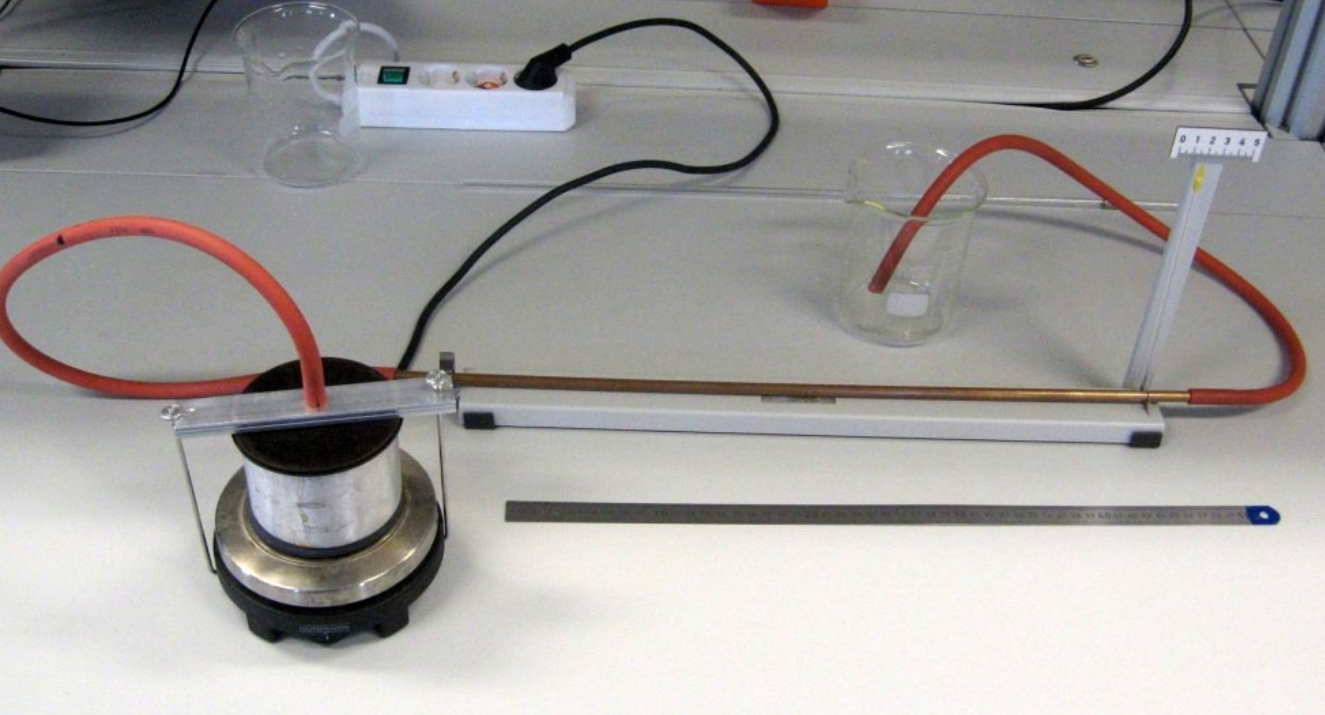
\includegraphics[width=12cm]{Abbildungen/aufbau_warmeausdehnung2}
\centering
\caption{Versuchsaufbau Wärmeausdehnung \cite{anl}}
\centering
\label{fig:bindungsenergie}
\end{figure}

\subsubsection{Durchführung}
Die Länge des Rohres im Kaltzustand, sowie die Maße des Zeigers werden gemessen und dokumentiert.
Anschließend wird die Kochplatte eingeschaltet, sodass Wasserdampf entsteht, welcher das Rohr auf etwa 100°C erhitzt.
Die auf der Skala angezeigte Änderung wird ebenfalls dokumentiert.
Der Versuch wird anschließend für ein Glasrohr wiederholt.

\subsection{Teil B: Mischtemperatur}
Der Versuch besteht aus zwei Teilen: \\

Im ersten Teil wird mit der Waage 200 g Wasser abgemessen und dessen Temperatur gemessen. In einem isolierten Behälter wird dies nun mit 20 g bis 40 g Eis gemischt und anschließend (nach dem Schmelzen) die Mischtemperatur gemessen. \\

Im zweiten Teil wird einem Eis-Wasser-Gemisch 20 g bis 40 g Wasser entnommen und dieses erneut mit 200 g warmen Wasser gemischt. Die genaue Temperatur des wärmeren Wassers wurde vorher ebenfalls dokumentiert. Nach dem Mischen wird ebenfalls die die Mischtemperatur gemessen.\\

\newpage
\section{Auswertung Versuch}

\subsection{Teil A: Wärmeausdehnung}

Für die Temperatur des Wasserdampfes bzw. der Temperatur des Rohres wird $\vartheta_E = 100\; ^\circ C \pm 5\; ^\circ C$ angenommen, da Wasser bei normalem Druck nicht weiter erhitzt werden kann. Ebenfalls zur Messunsicherheit trägt bei, dass in dem Schlauch ebenfalls Temperatur verloren geht. Als Anfangstemperatur des Rohres wird die Raumtemperatur von $\vartheta_A = 25\; ^\circ C \pm 3\; ^\circ C$ angenommen.\\

Als Temperaturänderung ergibt sich daraus $\Delta \vartheta = 75\; ^\circ C \pm 8\; ^\circ C$

Für die Zeigegeometrie wurden folgende Werte bestimmt.

\begin{figure}[H]
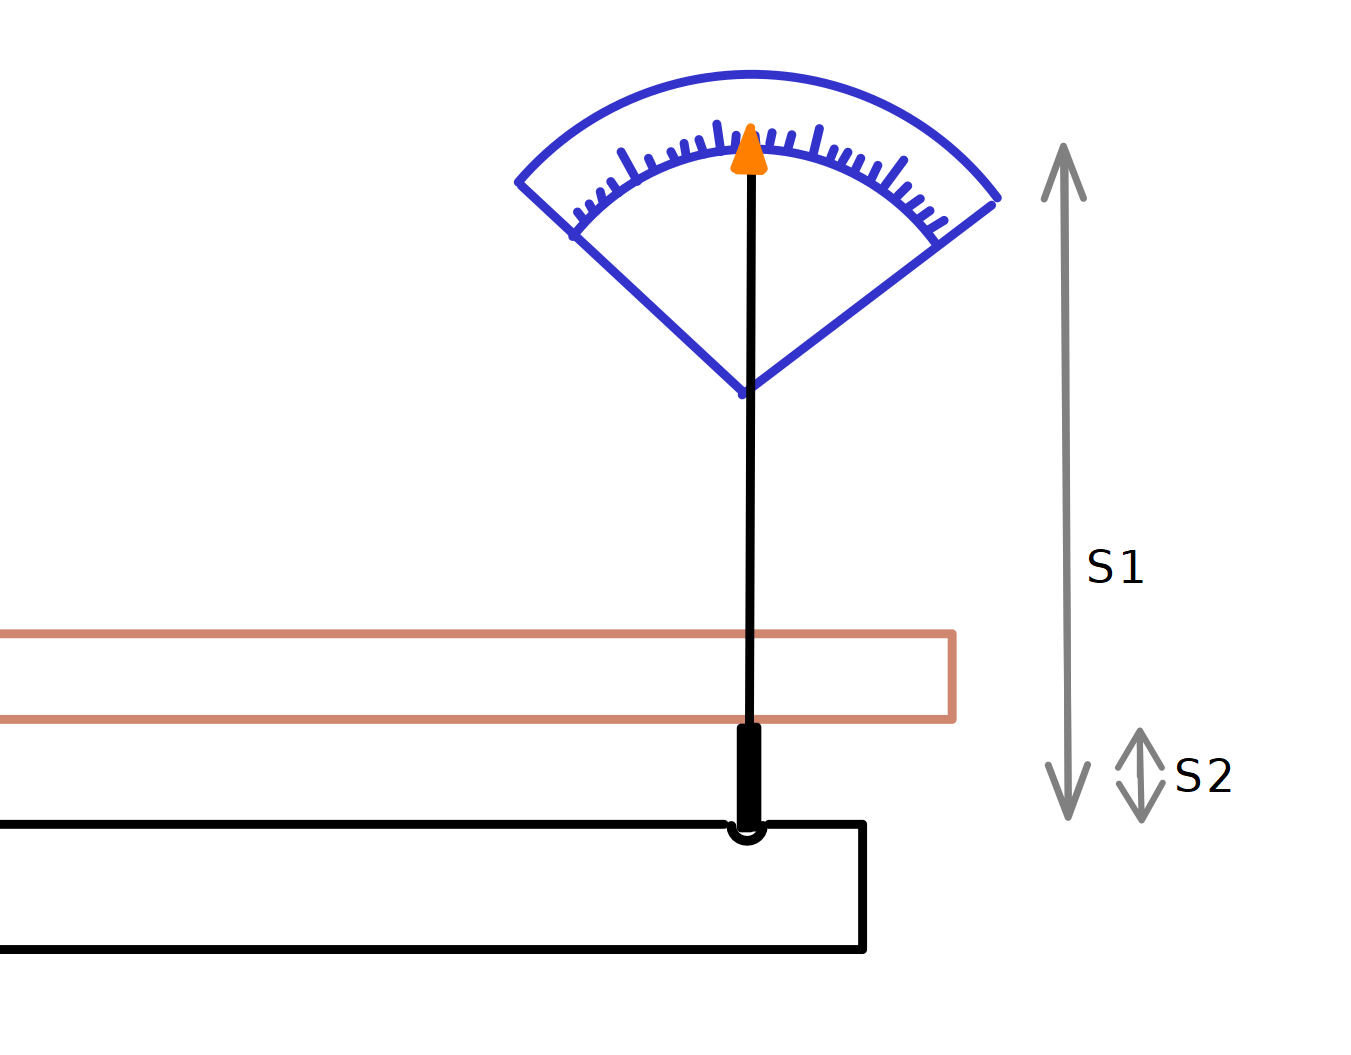
\includegraphics[width=12cm]{Abbildungen/aufbau_warmeausdehnung}
\centering
\caption{Zeigergeometrie des Messaufbaus}
\centering
\label{fig:bindungselektronen}
\end{figure}

\begin{align*}
S_1 \qquad 	& = (19 \pm 1)\;mm \\
S_2	\qquad 	& = (4 \pm 0,05)\;mm
\end{align*}

Da es sich bei dem Zeiger um eine Art "Hebel" handelt kann die tatsächliche Auslenkung und deren Unsicherheit bestimmt werden mit:

\begin{align}
\Delta L = \Delta x \cdot \frac{S_2}{S_1}
\end{align}

\textit{Fehlerrechnung:}

\begin{align*}
\frac{\partial}{\partial \Delta x} \Delta L &= \frac{S_2}{S_1} \\
\frac{\partial}{\partial S_2} \Delta L      &= \Delta x \cdot \frac{1}{S_1} \\
\frac{\partial}{\partial S_1} \Delta L      &= - \Delta x \cdot \frac{S_2}{S_1^2}
\end{align*}

\begin{align*}
U_{\Delta L} = \bigg | \frac{\partial}{\partial \Delta x} \Delta L \bigg | \cdot U_{\Delta x} + \bigg | \frac{\partial}{\partial S_2} \Delta L \bigg | \cdot U_{S_2} + \bigg | \frac{\partial}{\partial S_1} \Delta L \bigg | \cdot U_{S_1}
\end{align*}

Die Gleichung zur Wärmeausdehnung nach $\alpha$ umgestellt:

\begin{align}
\alpha = \frac{\Delta L}{L_0 \cdot \Delta \vartheta}
\end{align}

\textit{Fehlerrechnung:}

\begin{align*}
\frac{\partial}{\partial \Delta L} \alpha         &= \frac{1}{L_0 \cdot \Delta \vartheta} \\
\frac{\partial}{\partial L_0} \alpha              &= - \frac{\Delta L}{L_0^2 \cdot \Delta \vartheta} \\
\frac{\partial}{\partial \Delta \vartheta} \alpha &= - \frac{\Delta L}{L_0 \cdot \Delta \vartheta^2}
\end{align*}

\begin{align*}
U_{\alpha} = \bigg | \frac{\partial}{\partial \Delta L} \alpha \bigg | \cdot U_{\Delta L} + \bigg | \frac{\partial}{\partial L_0} \alpha \bigg | \cdot U_{L_0} + \bigg | \frac{\partial}{\partial \Delta \vartheta} \alpha \bigg | \cdot U_{\Delta \vartheta}
\end{align*}

\subsubsection{Kupferrohr}

Gemessen wurde eine Anfangslänge von $L_0 = 495 \;mm \pm 5 \;mm $ und eine Zeigeauslenkung von $\Delta x = 35 \;mm \pm 1 \;mm$.\\

daraus ergibt sich:

\begin{align*}
\Delta L = (7,4\pm2,1)\;mm
\end{align*}

und

\begin{align*}
\alpha = (20,0\pm8,1)\;\frac{10^{-5}}{ ^\circ C}
\end{align*}

\subsubsection{Glasrohr}

Gemessen wurde eine Anfangslänge von $L_0 = 495 \;mm \pm 5 \;mm $ und eine Zeigeauslenkung von $\Delta x = 16 \;mm \pm 1 \;mm$.\\

daraus ergibt sich:

\begin{align*}
\Delta L = (3,4\pm1,1)\;mm
\end{align*}

und

\begin{align*}
\alpha = (9,2\pm4,1)\;\frac{10^{-5}}{ ^\circ C}
\end{align*}


\subsection{Teil B: Mischtemperatur}

\subsubsection{Mischung von Eiswasser und Wasser}
Der Versuch wurde mit folgenden Werten durchgeführt:

\begin{align*}
\text{Masse Eiswasser} \quad m_1 &= (30,33\pm0,5)\;g \\
\text{Masse warmes Wasser} \quad m_2 &= (200,39\pm0,5)\;g \\
\text{Temp. warmes Wasser} \quad \vartheta_2 &= (18\pm1)\; ^\circ C
\end{align*}

Dabei wurde eine Mischtemperatur von $\vartheta_{M, \textit{exp.}} = (15\pm1)\; ^\circ C$ gemessen \\

\textbf{Berechnung Mischtemperatur}

\begin{align}
\vartheta_{M, \textit{theor.}} = \frac{\vartheta_2 \cdot m_2}{m_1 + m_2}
\end{align}

\textit{Fehlerrechnung:}

\begin{align*}
\frac{\partial}{\partial \vartheta_2} \vartheta_{M, \textit{theor.}} &= \frac{m_2}{m_1 + m_2} \\
\frac{\partial}{\partial m_2} \vartheta_{M, \textit{theor.}} &= \frac{\vartheta_2 \cdot m_1}{(m_1 + m_2)^2} \\
\frac{\partial}{\partial m_1} \vartheta_{M, \textit{theor.}} &= - \frac{\vartheta_2 \cdot m_2}{(m_1 + m_2)^2}
\end{align*}

\begin{align*}
U_{\vartheta_{M, \textit{theor.}}} = \bigg | \frac{\partial}{\partial \vartheta_2} \vartheta_{M, \textit{theor.}} \bigg | \cdot U_{\vartheta_2} + 
									\bigg | \frac{\partial}{\partial m_2} \vartheta_{M, \textit{theor.}} \bigg | \cdot U_{m_2} +
									\bigg | \frac{\partial}{\partial m_1} \vartheta_{M, \textit{theor.}} \bigg | \cdot U_{m_1}
\end{align*}

\begin{align*}
\vartheta_{M, \textit{theor.}} = (15,63\pm0,91)\; ^\circ C \\
\vartheta_{M, \textit{exp.}} = (15\pm1)\; ^\circ C
\end{align*}

\subsubsection{Mischung von Eis und Wasser}

Der Versuch wurde mit folgenden Werten durchgeführt:

\begin{align*}
\text{Masse Eis} \quad m_1 &= (34,43\pm0,5)\;g \\
\text{Masse warmes Wasser} \quad m_2 &= (200,55\pm0,5)\;g\\
\text{Temp. warmes Wasser} \quad \vartheta_2 &= (19\pm1)\; ^\circ C
\end{align*}

Dabei wurde eine Mischtemperatur von $\vartheta_{M, \textit{exp.}} = (8\pm1)\; ^\circ C$ gemessen \\

\textbf{Berechnung Mischtemperatur}
Konstanten: $q_S = 334\;\frac{kJ}{kg}$ und $c_W = 4,190\;\frac{kJ}{kg ^\circ C}$ \\

\begin{align}
\vartheta_{M, \textit{theor.}} = \frac{\vartheta_2 \cdot c \cdot m_2 - m_1 \cdot q_S}{c \cdot (m_1 + m_2)}
\end{align}

\textit{Fehlerrechnung:}

\begin{align*}
\frac{\partial}{\partial \vartheta_2} \vartheta_{M, \textit{theor.}} &= \frac{m_2}{m_1 + m_2} \\
\frac{\partial}{\partial m_2} \vartheta_{M, \textit{theor.}} &= \frac{m_1 \cdot (c \cdot \vartheta_2 + q_S)}{c \cdot (m_2+m_1)^2} \\
\frac{\partial}{\partial m_1} \vartheta_{M, \textit{theor.}} &= -\frac{m_2 \cdot (c \cdot \vartheta_2 + q_S)}{c\cdot(m_1+m_2)^2}
\end{align*}

\begin{align*}
U_{\vartheta_{M, \textit{theor.}}} = \bigg | \frac{\partial}{\partial \vartheta_2} \vartheta_{M, \textit{theor.}} \bigg | \cdot U_{\vartheta_2} + 
									\bigg | \frac{\partial}{\partial m_2} \vartheta_{M, \textit{theor.}} \bigg | \cdot U_{m_2} +
									\bigg | \frac{\partial}{\partial m_1} \vartheta_{M, \textit{theor.}} \bigg | \cdot U_{m_1}
\end{align*}

\begin{align*}
\vartheta_{M, \textit{theor.}} = (4,5\pm1,1)\; ^\circ C \\
\vartheta_{M, \textit{exp.}} = (8\pm1)\; ^\circ C
\end{align*}

\newpage
\section{Wertung/Fazit}
\subsection{Teil A: Wärmeausdehnung}
Beim Versuch Wärmeausdehnung waren sowohl beim Glasrohr, als auch beim Kupferrohr eine Längen-\ änderung anhand des Zeigers deutlich zu erkennen. Die daraus resultierenden berechneten Werte stimmten im Rahmen der Messunsicherheit mit den Literaturwerten überein,auch wenn die berechnete Messunsicherheit sehr groß ist. Die Differenz der berechneten Werte mit den Literaturwerten bzw. die sehr große Messunsicherheit ist darauf zurückzuführen, dass der Wasserdampf in dem Schlauch aber auch im Rohr einiges abkühlt. Auch ist einiges an Ungenauigkeit beim Ablesen mit dem Zeiger entstanden.
\subsection{Teil B: Mischtemperatur}
Auch hier stimmen die gemessenen Werte gut mit den berechneten Werten überein. Im Falle des ersten Versuches ist das Ergebnis sogar sehr nah an dem tatsächlichen Wert dran. Bei dem zweiten Versuch mit dem Eis - warmen Wassergemisch ist dies leider nicht der Fall, der gemessene Wert und der tatsächliche Wert gehen einiges auseinander. Eine mögliche Erklärung für die größere Abweichung beim Eis - warmen Wassergemisch ist die größere Differenz der Mischtemperatur gegenüber der Raumtemperatur, wodurch sich das Gemisch stärker erwärmt als erwartet.

\newpage

\bibliography{literatur}

\label{LastPage}

\end{document}
%%% Local Variables:
%%% mode: latex
%%% TeX-master: t
%%% End:
